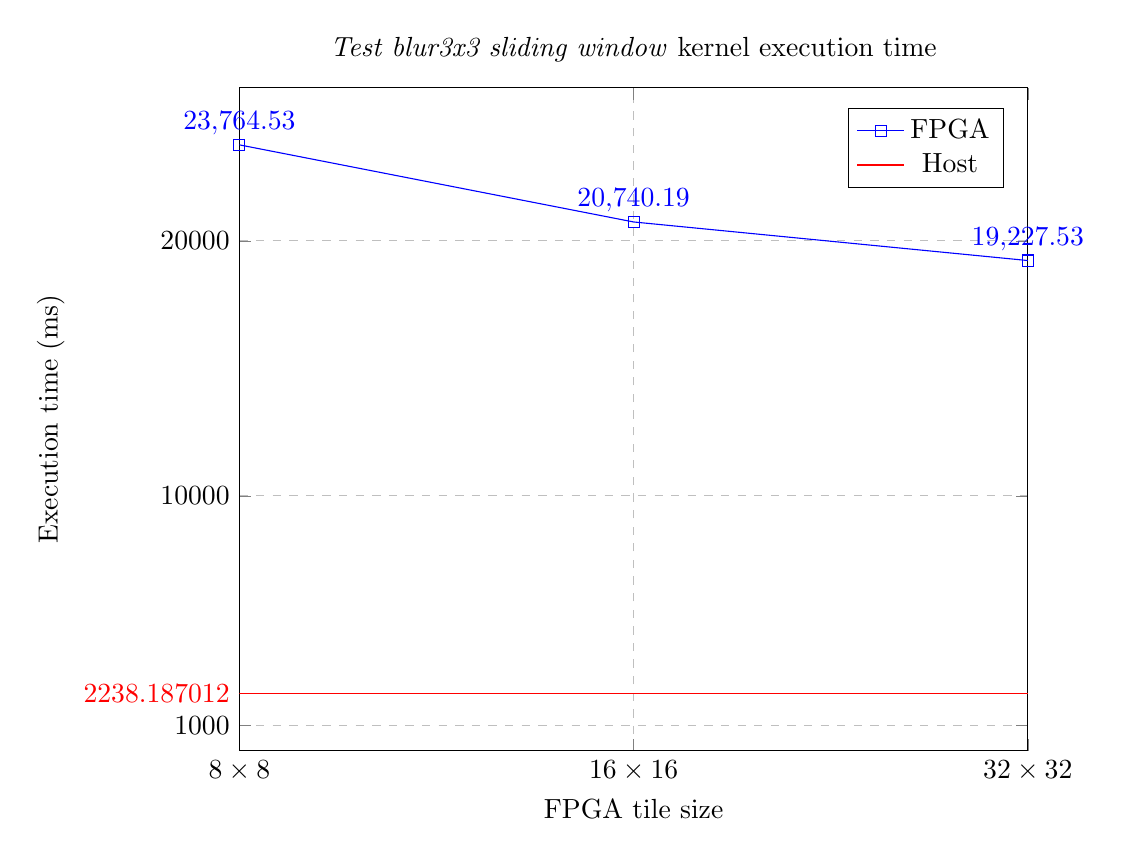
\begin{tikzpicture}
\begin{axis}[
    title={\textit{Test blur3x3 sliding window} kernel execution time},
    xlabel={FPGA tile size},
    ylabel={Execution time (ms)},
    xmin=1, xmax=3,
    ymin=0, ymax=26000,
    xticklabels={$8 \times 8$, $16 \times 16$, $32 \times 32$},
    xtick={1,2,3},
    ytick={1000,2238.187012,10000,20000},
    yticklabels={1000,\textcolor{red}{2238.187012},10000,20000},
    legend pos=north east,
    xmajorgrids=true,
    ymajorgrids=true,
    grid style=dashed,
    height=10cm,
    ytick scale label code/.code={}
]
\addplot[color=blue,mark=square, nodes near coords]
    coordinates {
        (1, 23764.525391) (2, 20740.193359) (3, 19227.529297)
    };
    \addlegendentry{FPGA}

\addplot[color=red]
    coordinates {
        (1, 2238.187012) (2, 2238.187012) (3, 2238.187012)
    };
    \addlegendentry{Host}

\end{axis}
\end{tikzpicture}
